\documentclass[12pt]{article}

\usepackage[affil-it]{authblk}
\usepackage[shortlabels]{enumitem}
\usepackage[utf8]{inputenc}
\usepackage{algorithm, algorithmicx, algpseudocode}
\usepackage{amsfonts, amsthm, amsmath, amssymb}
\usepackage{color}
\usepackage{cancel, textcomp}
\usepackage{enumerate}
\usepackage[mathscr]{euscript}
\usepackage{fancyhdr, fancyvrb}
\usepackage{fullpage}
\usepackage[left=0.5in,right=0.5in,headsep=0.5in,headheight=0.5in]{geometry}
\usepackage{graphicx}
\usepackage{hyperref}
\usepackage{latexsym}
\usepackage{mathtools}
\usepackage{minted}
\usepackage{times}
\usepackage{xcolor}
\usepackage{physics}
\usepackage{tikz-cd}
\usepackage[warnunknown, fasterrors, mathletters]{ucs}
\usepackage[nointegrals]{wasysym}

\newcommand{\hw}[2]{
    \noindent
    \begin{center}
        \framebox{
            \vbox{
                \hbox to 7in { {\bf MATH 470: Communications and Cryptography } \hfill  }
                \vspace{2mm}
                \hbox to 7in { {\Large \hfill Homework #1\hfill} }
                \vspace{2mm}
                \hbox to 7in { {\it Due date: #2 \hfill Name: Huy Lai } }
            }
        }
    \end{center}
    \vspace*{4mm}
}

\newcounter{prob}
\setcounter{prob}{0}
\newcounter{subprob}
\setcounter{subprob}{0}

\newcommand{\problem}{\setcounter{subprob}{0}\stepcounter{prob}{\noindent\textbf{Problem \theprob.}}\ }
\newcommand{\subproblem}{\stepcounter{subprob}{\noindent\textbf{Subproblem \thesubprob.}}\ }
\newcommand{\solution}{\noindent\textbf{Solution:}\newline}

\newcommand{\babc}{\begin{enumerate}[a)]}
\newcommand{\eabc}{\end{enumerate}}

\everymath{\displaystyle}

\setlength{\parskip}{.1in}
\setlength{\headheight}{15pt}
\setlength{\topmargin}{0pt}

\fancyhf{}
\pagestyle{fancy}
\lhead{MATH 470: Communications and Cryptography}
\rhead{Texas A\&M University}
\cfoot{\thepage}


\begin{document}
\thispagestyle{empty}
\hw{2}{7 September 2023}

\problem For each of the $\gcd(a,b)$ values in Exercise 1.9, use the extended Euclidean algorithm (Theorem 1.11) to find integers $u$ and $v$ such that $au+bv=\gcd(a,b)$. Let $a=291$ and $b=252$

\solution
\begin{table}[!ht]
    \centering
    \begin{tabular}{|c|c|c|c| }
        \hline
        $q$ & $r$   & $u$  & $v$   \\
        \hline
            & $291$ & $1$  & $0$   \\
            & $252$ & $0$  & $1$   \\
        $1$ & $39$  & $1$  & $-1$  \\
        $6$ & $18$  & $-6$ & $7$   \\
        $2$ & $3$   & $13$ & $-15$ \\
            & $0$   & $u$  & $v$   \\
        \hline
    \end{tabular}
    \caption{Extended Euclidean Algorithm}
\end{table}
\[
    u=13,v=-15
\]

\newpage
\problem Let $a_1,a_2,\dots,a_k$ be integers with $\gcd(a_1,a_2,\cdots,a_k)=1$ i.e., the largest positive integer dividing all of $a_1,a_2,\dots,a_k$ is 1. Prove that the equation
\[a_1u_1+a_2u_2+\cdots+a_ku_k=1\]
has a solution in integers $u_1,u_2,\dots,u_k$. (\textit{Hint}. Repeatedly apply the extended Euclidean algorithm, Theorem 1.11. You may find it easier to prove a more general statement in which $\gcd(a_1,\dots,a_k)$ is allowed to be larger than 1.)

\solution
Proof by Induction
\begin{proof}
    Base case: $k=1$\\
    $a_1\cdot1=\gcd(a_1)$

    \noindent
    $k=2$\\
    This is proven by the Extended Euclidean Algorithm

    \noindent
    Inductive Hypothesis: Assume $\forall k\geq3$ that
    \[a_1u_1+a_2u_2+\cdots+a_{k-1}u_{k-1}=\gcd(a_1,a_2,\cdots,a_{k-1})\]
    Let $b=\gcd(a_1,\cdots,a_{k-1})$.\\
    Apply the Extended Euclidean algorithm to $b$ and $a_k$, this gives the solution
    \[
        bu+a_kv=\gcd(b,a_k)
    \]

    \noindent
    Multiplying the Inductive Hypothesis by $v$ results in
    \begin{align*}
        a_1u_1v+a_2u_2v+\cdots+a_{k-1}u_{k-1}v & = \gcd(a_1,a_2,\cdots,a_{k-1})v                    \\
                                               & = bv \text{ by the definition of }b                \\
                                               & = -a_kv+\gcd(b,a_k) \text{ by rearranging the EEA}
    \end{align*}

    \noindent
    Adding $a_kv$ to both sides of this equation results in
    \[
        a_1u_1+a_2u_2+\cdots+a_{k-1}u_{k-1}+a_kv=\gcd(b,a_k)
    \]

    \noindent
    Since $b=\gcd(a_1,\cdots,a_{k-1})$,
    \begin{flalign*}
        \gcd(b,a_k) & = \gcd(\gcd(a_1,\cdots,a_{k-1}),a_k) & \\
                    & = \gcd(a_1,a_2,\cdots,a_{k_1},a_k)   &
    \end{flalign*}
\end{proof}

\newpage
\problem Find all values of $x$ between $0$ and $m-1$ that are solutions of the following congruences. (\textit{Hint}. If you can’t figure out a clever way to find the solution(s), you can just substitute each value $x=1,x=2,\dots,x=m-1$ and see which ones work.)

\subproblem $x^2\equiv 3\mod 11$

\solution
The squares modulo 11 are $\{0,1,4,9,5,3,3,5,9,4,1\}$\\
Therefore, $5^2\equiv 3\mod{11}$ and $6^2\equiv 3\mod{11}$

\subproblem $x^2\equiv 2\mod 13$

\solution
The squares modulo 13 are $\{0,1,4,9,3,12,10,10,12,3,9,4,1\}$\\
Therefore, $x^2\equiv 2\mod 13$ has no solutions

\problem Suppose that $g^a\equiv 1\mod m$ and that $g^b\equiv 1\mod m$. Prove that
\[g^{\gcd(a,b)}\equiv 1\mod m\]

\solution
According to the Extended Euclidean Algorithm, $\exists u,v\in\mathbb{Z}$ such that $au+bv=\gcd(a,b)$. Then
\[g^{\gcd(a,b)}=g^{au+bv}=(g^a)^u\cdot(g^b)^v\equiv1^u\cdot1^v\equiv 1\mod{m}\]
Since $g^a\equiv1\mod{m}$ and $g^b\equiv1\mod{m}$, the above equation holds.

\newpage
\problem Let $m\in\mathbb{Z}$

\subproblem Suppose that $m$ is odd. What integer between 1 and $m-1$ equals $2^{-1}\mod{m}$?

\solution
Since $m$ is odd, then $\frac{m+1}{2}$ must also be an integer, since $m+1$ is an even number. Therefore
\[2\cdot\frac{m+1}{2}=m+1\equiv1\mod{m}\]

\noindent
Therefore $\frac{m+1}{2}=2^{-1}\mod{m}$

\subproblem More generally, suppose that $m\equiv 1\mod b$. What integer between 1 and $m-1$ is equal to $b^{-1}\mod m$?

\solution
The assumption that $m=1\mod{b}\rightarrow b\mid (m-1)$ by proposition.\\
By the definition of division, $b\mid (m-1)\rightarrow\exists x\in\mathbb{Z}$ such that $m-1=bx$. This requires that $\frac{m-1}{b}\in\mathbb{Z}$\\
Multiplying this fraction by $b$ results in
\[b\cdot\frac{m-1}{b}=m-1\equiv-1\mod{m}\]
Multiplying this result by $-1$ results in
\[b\cdot\frac{1-m}{b}=1-m\equiv1\mod{m}\]
However, $\frac{1-m}{b}$ is negative, but we can add multiples of $m$ without effecting the value of modulo $m$. As a result, $\frac{1-m}{b}+m=\frac{1+(b-1)m}{b}$ is an integer and more importantly is congruent to $1\mod{m}$.

\noindent
Therefore, $\frac{1+(b-1)m}{b}=b^{-1}\mod{m}$

\newpage
\problem Consider the congruence
\[
    ax\equiv c\mod m
\]
Prove that there is a solution if and only if $\gcd(a,m)\mid c$.

\solution
First we prove that if $ax\equiv c\mod{m}$ has a solution, then $\gcd(a,m)\mid c$
\begin{proof}
    Let $x$ be a solution to the congruency $ax\equiv c\mod{m}$.\\
    By definition of congruence and divisibility
    \[\exists y\in\mathbb{Z},ax=c+my\]
    Since $\gcd(a,m)\mid a$ and $\gcd(a,m)\mid m$ $gcd(a,m)\mid ax-my$ by proposition on linear combinations
\end{proof}

\noindent
Next we prove that if $\gcd(a,m)\mid c$, then $ax\equiv c\mod{m}$ has a solution
\begin{proof}
    According to the Extended Euclidean Algorithm, $\exists u,v\in\mathbb{Z}$ such that
    \[au+mv=\gcd(a,m)\]
    $\gcd(a,m)|c\rightarrow(au+mv)|c$\\
    By definition of divisibility, $\exists y\in\mathbb{Z}$ such that $c=(au+mv)y$\\
    Rearranging this equation results in $mvy=c-auy\Rightarrow -mvy=auy-c$ or equivalently $mY=aX-c$ where $X=uy,Y=-vy$\\
    Since $X,Y\in\mathbb{Z}$, the definition of divisibility implies that $m\mid (aX-c)$.\\
    By one of the modular propositions, $m\mid (aX-c)\rightarrow aX\equiv c\mod{m}$.\\
    This proves that if $\gcd(a,m)\mid c$, then $ax\equiv c\mod{m}$ has a solution
\end{proof}

\newpage
\problem Let
\begin{flalign*}
    a & = 1234567890123456789012345678901234567890123456789012345678901234567890123456789, & \\
    b & = 234567890123456789012345678901234567890123456789012345678901234567890123456789   &
\end{flalign*}
Find the inverse of $a$ modulo $b$ AND the inverse of $b$ modulo $a$ (as an integer between 0 and $b-1$ in the first case, and as an integer between 0 and $a-1$ in the second case), or explain why these inverses do not exist.

\solution
\inputminted{python}{modInverse.py}

\begin{figure}[!ht]
    \centering
    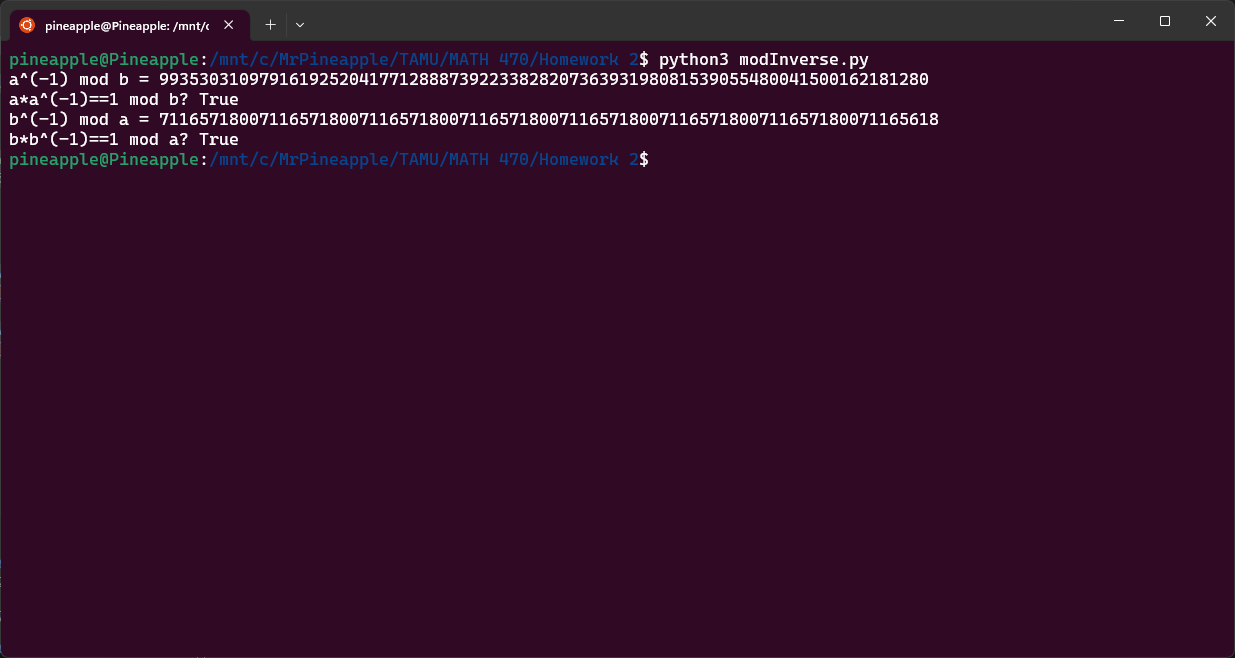
\includegraphics[width=0.9\textwidth]{Problem 7.png}
    \caption{Output}
\end{figure}

\end{document}